\documentclass{ctexart}
\usepackage{amsmath}
\usepackage{circuitikz}
\usepackage{caption}
\newcommand\ohm{\ \Omega}
\newcommand\mV{\ \mathrm{mV}}
\newcommand\mA{\ \mathrm{mA}}
\newcommand\Hz{\ \mathrm{Hz}}
\newcommand\kHz{\ \mathrm{kHz}}

\title{RLC谐振实验报告}
\author{* *}

\begin{document}
    \maketitle
    \section{实验简介}
    在本实验中, 我们测量RLC串联电路的谐振特性以及RLC串联电路的相频特性与幅频特性。
    实验电路图连接如图一,通过隔离变压器解决示波器与信号发生器共地问题,利用双频道示波器
    以及万用表的电压位测量电路以及标准电阻上的电流。

    在本实验中:
    \begin{align}
        R_0 &= 100\  \Omega \\
        L_0 &= 0.1\  \mathrm{H} \\
        r_L &= 18.114\ \Omega \\
        C_0 &= 0.5\  \mu\mathrm{F}
    \end{align}

    \begin{figure}
        \centering
        \begin{circuitikz}[american]
            \draw (0, 0) -- ++(1, 0) 
                node[transformer, anchor=A1](trs){}
                (trs.A2) -- ++ (-1,0) to[sV] (0, 0);
            \draw (trs.B2) -- ++(0.5, 0) to[R] ++(1, 0) -- ++(1, 0) coordinate(l_0)
                to[L, name=l] ++(1, 0) -- ++(1, 0)
                to[C] ++(1, 0) -- ++(0.5, 0) coordinate(c_0) -- ++(0, 2) -- (trs.B1);
                \draw[thick] (l.core west) -- (l.core east);
            \draw(trs.B2) -- node[ground]{} ++(0, -1);
            \draw($(l_0)-(0.5, 0)$) to[short, -o] ++(0, -1) node[below]{CH2};
            \draw(c_0) to[short, -o] ++(0, -1) node[below]{CH1};
        \end{circuitikz}
        \caption{实验电路图}
    \end{figure}

    \section{测定谐振参数}
    调整信号发生器频率,使得两频道的李萨如图形为一条直线时,即为RLC系统的谐振频率。在测量谐振频率时,应合理调整
    示波器电压档位,并估计谐振频率的不确定度。
    在实验中,测得谐振频率与极限不确定度:
    \begin{align}
        f_0 &= 2245.8 \ \mathrm{Hz} \\
        \mathrm{e}_f &= 0.6 \ \mathrm{Hz}
    \end{align}
    因此有:
    \begin{equation}
        f_0 = 2245.8 \pm 0.35 \ \mathrm{Hz} 
    \end{equation}
    在谐振时,测得电路上总电压以及电感、电容上电压为:
    \begin{align}
        U &= 214.33 \pm 0.01 \ \mathrm{mV} \\
        U_L &= 2.3288 \pm 0.0003 \ \mathrm{V} \\
        U_C &= 2.3195 \pm 0.0004 \ \mathrm{V}
    \end{align}
    考虑到电容上耗散电阻远小于电感上耗散电阻, 利用电容上电压计算得到:
    \begin{equation}
        Q_2 = \frac{U_C}{U} = 10.822 \pm 0.002
    \end{equation}
    电路中总直流电阻为:
    \begin{equation}
        R_D = R_0 + r_L = 118.114 \ohm
    \end{equation}
    利用储能法计算品质因数:
    \begin{equation}
        Q_1 = \frac{\omega_0 L}{R_D} = 11.945 \pm 0.002
    \end{equation}

    两种方法计算出的品质因数远远超出可接受的误差范围内,因此我们可以得到结论:电路中的交流耗散不可忽略。
    电路中的交流耗散主要分为两部分,电感中磁铁芯的磁滞现象带来一项铁组,高频时导线内的趋肤效应带来一项铜阻,两项相加即为总的交流电阻。
    计算可得回路中的交流电阻约为:
    \begin{equation}
        r_A = 12 \ohm
    \end{equation}

    \section{测量RLC系统的特性曲线}
    在测量相频特性曲线时,利用示波器获得标准电阻以及总电压上的波形曲线,合理调整量程后利用等相位点处时间差计算相位偏移。
    在具体计算中,利用波形与$x$轴交点作为等相位点。
    \begin{figure}[h]
        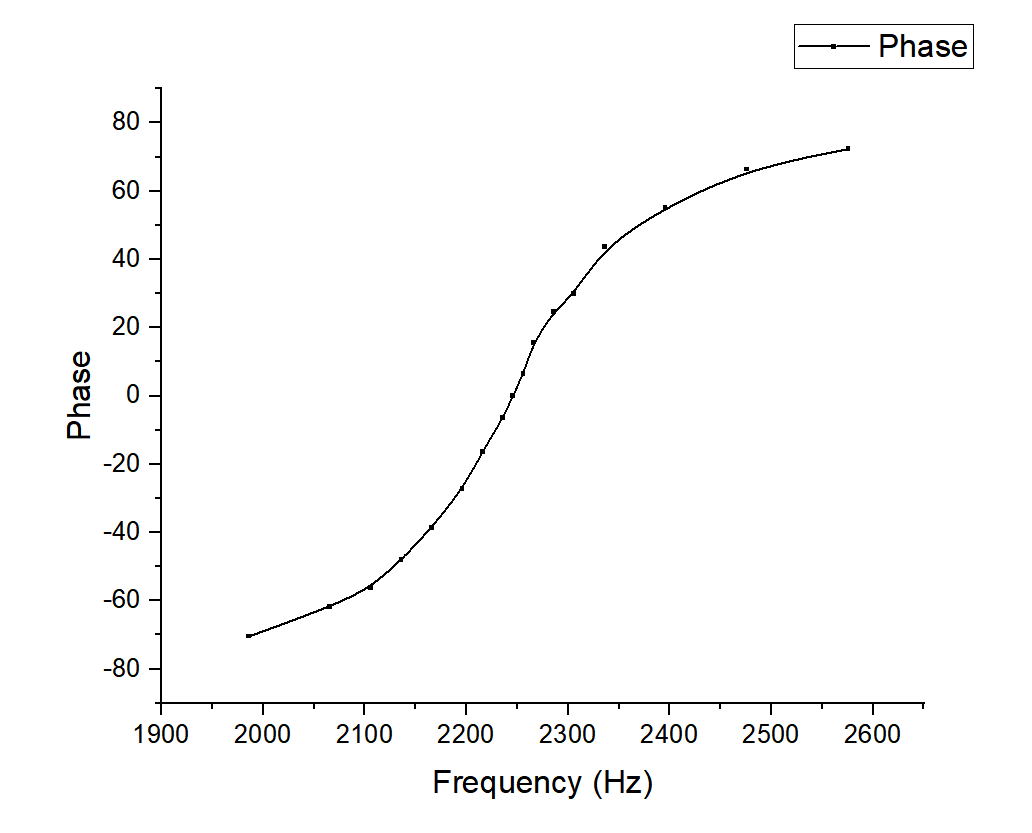
\includegraphics[width=\textwidth]{rlc_1.png}
        \caption{相频数据}
    \end{figure}

    在测量幅频特性曲线时,假定电路对电压线性响应,保持信号源电压不变,用万用表交流电压档测量总电压以及标准电阻上电压,
    归一后得到电流$I_\mathrm{norm}$。

    归一化后测量峰值为:
    \begin{align}
        i_p &= 77.823 \ \mathrm{mA} \\
        i' &= \frac{i_p}{\sqrt{2}} = 55.029 \ \mathrm{mA}
    \end{align}

    拟合后获得的两交点分别位于:
    \begin{align}
        f_1 &= 2145.6 \ \mathrm{Hz} \\
        f_2 &= 2350.5 \ \mathrm{Hz} \\
        \Delta f &= f_2 - f_1 = 204.9 \ \mathrm{Hz}
    \end{align}

    因而利用通频特性计算得到的品质因数为:
    \begin{equation}
        Q_3 = \frac{f_0}{\Delta f} = 10.96
    \end{equation}

    该数值与$Q_2$的结果相当接近。

    \begin{figure}[h]
        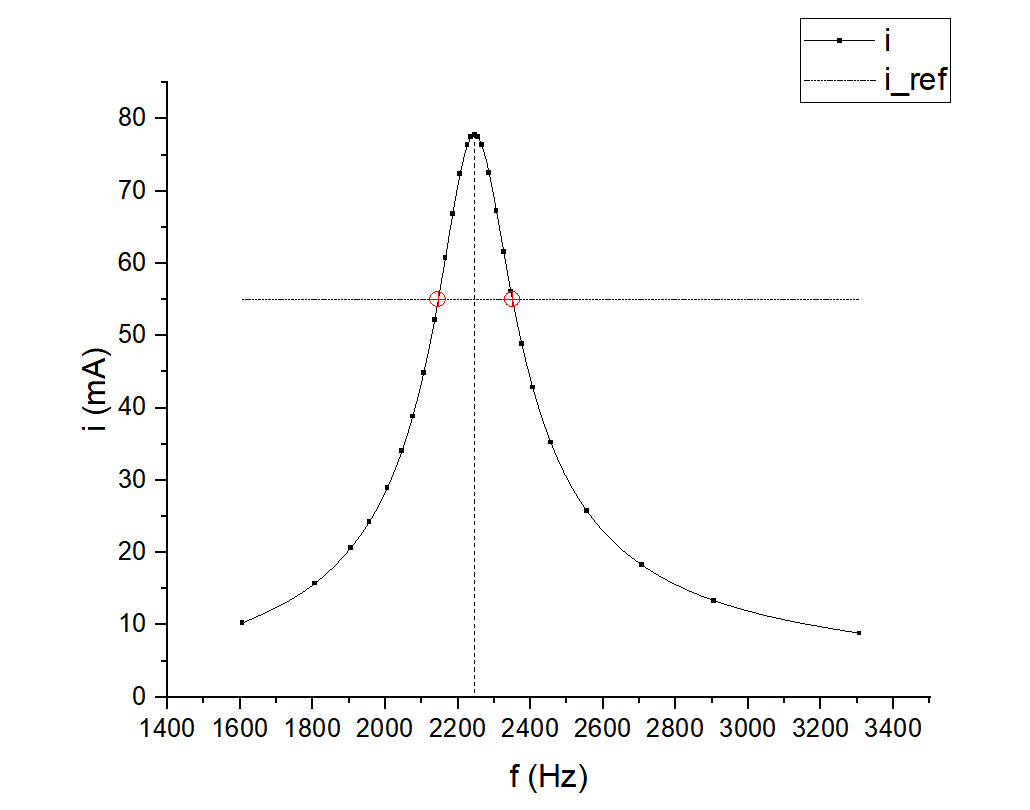
\includegraphics[width=\textwidth]{rlc_2.png}
        \caption{幅频数据}
    \end{figure}

    % Table generated by Excel2LaTeX from sheet 'phi-f'
    \begin{figure}[p]
        \centering
        \begin{minipage}[t]{0.45\textwidth}
            \begin{tabular}{||c|c|c||}
                \hline
                $f(\mathrm{Hz})$ & $1/\Delta T(\mathrm{kHz})$ & $\phi$ \\
                \hline
                1985.8 & -10.15  & -70.43  \\
                2065.8 & -12.04  & -61.77  \\
                2105.8 & -13.51  & -56.11  \\
                2135.8 & -16.00  & -48.06  \\
                2165.8 & -20.20  & -38.60  \\
                2195.8 & -28.98  & -27.28  \\
                2215.8 & -48.78  & -16.35  \\
                2235.8 & -125.0  & -6.44  \\
                2245.8 & $\infty$  & 0.00  \\
                2255.8 & 125.0  & 6.50  \\
                2265.8 & 52.63  & 15.50  \\
                2285.8 & 33.33  & 24.69  \\
                2305.8 & 27.77  & 29.89  \\
                2335.8 & 19.23  & 43.73  \\
                2395.8 & 15.62  & 55.22  \\
                2475.8 & 13.42  & 66.41  \\
                2575.8 & 12.82  & 72.33  \\
                3045.8 & 12.82  & 85.53  \\
                \hline
            \end{tabular}%
            \captionsetup{type=table}
            \caption{相频数据}
            \quad $f$为信号发生器生成频率,$\Delta T$为等相位点时间间隔,相位计算公式为
            $\phi = f / (1/\Delta T)$.
        \end{minipage}
        \hfill
        \begin{minipage}[t]{0.45\textwidth}
            \begin{tabular}{||c|c|c|c||}
                \hline
                $f$ & $U$ & $U_R$ & $I_\textrm{norm}$ \\
                (Hz) & (mV) & (mV) & (mA) \\
                \hline
                1605.8 & 407.8 & 41.86  & 10.265  \\
                1805.8 & 427.4 & 67.36  & 15.760  \\
                1905.8 & 441.5 & 91.29  & 20.677  \\
                1955.8 & 448.3 & 108.61  & 24.227  \\
                2005.8 & 451.5 & 130.84  & 28.979  \\
                2045.8 & 446.6 & 152.05  & 34.046  \\
                2075.8 & 433.9 & 168.66  & 38.871  \\
                2105.8 & 409.2 & 183.57  & 44.861  \\
                2135.8 & 370.5 & 193.43  & 52.208  \\
                2165.8 & 321.2 & 195.32  & 60.809  \\
                2185.8 & 286.97  & 191.87  & 66.861  \\
                2205.8 & 256.01  & 185.31  & 72.384  \\
                2225.8 & 231.28  & 176.63  & 76.371  \\
                2235.8 & 221.78  & 171.81  & 77.469  \\
                2245.8 & 214.32  & 166.79  & 77.823  \\
                2255.8 & 208.73  & 161.71  & 77.473  \\
                2265.8 & 204.99  & 156.62  & 76.404  \\
                2285.8 & 202.11  & 146.65  & 72.559  \\
                2305.8 & 203.80  & 137.22  & 67.331  \\
                2325.8 & 208.34  & 128.45  & 61.654  \\
                2345.8 & 214.43  & 120.45  & 56.172  \\
                2375.8 & 224.63  & 109.80  & 48.880  \\
                2405.8 & 234.79  & 100.63  & 42.860  \\
                2455.8 & 250.04  & 88.08  & 35.226  \\
                2555.8 & 272.93  & 70.24  & 25.736  \\
                2705.8 & 294.14  & 53.92  & 18.331  \\
                2905.8 & 309.98  & 41.44  & 13.369  \\
                3305.8 & 325.32  & 28.82  & 8.859  \\
                \hline
            \end{tabular}%
            \captionsetup{type=table}
            \caption{幅频数据}
            \quad $f$为信号发生器生成频率,$U$为电路上总电压,$U_R$为标准电阻上电压。
            $I_\textrm{norm}$为总电压为$1$V时电流,计算公式为$I_\textrm{norm} = 100\times\frac{U}{U_R}$.
       
        \end{minipage}
    \end{figure}%
    \newpage

    \section{思考与收获}
    \subsection{Q表}
    Q表测量原理为$Q = U_c / U$,利用谐振时电容上的电压测得品质因数。
    测量时,调整可调电容使得$U_c / U$最大,该最大值即为谐振时的品质因数。
    用题中所给数据计算得到:
    \begin{align}
        L &= \frac{1}{4\pi^2 f^2 C} = 0.213 \ \mathrm{mH}\\
        Q &= \frac{u_c}{u} = 100 \\
        R_r &= \frac{2\pi f L}{Q} = 8.038 \ \ohm\\
    \end{align}
\end{document}